\documentclass[11pt] {article}
\usepackage{enumerate}
\usepackage{algorithm2e}
\usepackage{mcode}
\usepackage{listings}
\usepackage{graphicx}
\usepackage{epstopdf}
\usepackage{amsmath}
\usepackage{amssymb}


\newcommand{\inner}[2]{\left\langle #1,#2 \right\rangle}
\newcommand{\innerd}[2]{\left\langle \left\langle#1,#2 \right\rangle\right\rangle}
\newcommand{\real}{\ensuremath{\mathbb{R}}}
\newcommand{\s}{\ensuremath{\mathbb{S}}}
\newcommand{\ltwo}{\ensuremath{\mathbb{L}^2}}
\newcommand{\cC}{\ensuremath{\mathbb{C}}}

\newcommand{\Ftilde}{\widetilde{\cal F}}
\newcommand{\Fhat}{\widehat{\cal F}}

\author{Zhengwu Zhang}
\title{Midterm Project}

\begin{document} 

\maketitle
\newpage

\section{Problem Statement}

For a given observed noisy images, we want to noise the image with Bayesian analysis technology. Suppose we have a prior probability model and an observation model, and we want to get the posterior density from them. At last, we generate samples from the posterior. 

Moreover, I find that due to the model we are choosing, the posterior resampling is actually a kind of Gaussian smoothing, so I will compare posterior with Gaussian smoothing. And then we will analysis these smoothing with Blurring-Invariant Riemannian Metrics. 

\section{Methodology}

First of all we should build up the Models for our prior image and observation image. 

\noindent \textbf{Prior Model}: 

For a given image we can consider it to be a Markov Random Field (MRF), let say $m*n$ MRF.  We suppose the value of an element is only dependent on the values of its vertical and horizontal neighbors. Of course, these boundaries should be given special consideration.  Let the conditional density of a pixel be Gaussian with mean $\mu$ and variance $\delta_1^2$, $\mu$ is the mean of its neighbors. The prior model $f(I)$ is:

$$f(I_{i,j}|other pixel)=f(I_{i,j}|I_{i,j-1},I_{i,j+1},I_{i-1,j},I_{i+1,j})=N(\mu,\delta_1^2) $$

\noindent \textbf{Observation Model}: We use D to denote the noisy observation of image $I$, we build a model like this:

$$D=I+W$$

where $W$ is an independent normal random variable with mean zeros and variance $\delta_2^2$. We can use this function to specify the likelihood function $f(D|I)$ for the observation image $D$

\noindent \textbf{Posterior Density}: 

With the Bayesian theory, Posterior density can be written:

$$f(I|D) =c*f(D|I)*f(I)$$ where $c$ is just a normalization constant. 

Then the full conditional posterior density can be written as:

$$f(I|D)=f(I_{i,j}|D_{i,j},I_{i,j-1},I_{i,j+1},I_{i-1,j},I_{i+1,j})=N(\mu,\delta_1^2)N(D_{i,j},\delta_2^2)$$

We can see from the full conditional posterior density function that it is the product of two Gaussian. Actually the product of two Gaussian is another Gaussian.  let's say 

$$N(\mu,\sigma^2)=N(\mu_1,\sigma_1^2)*N(\mu_2,\sigma_2^2)$$

Then $\mu=\frac{\mu_1\sigma_2^2+\mu_2\sigma_1^2}{\sigma_2^2+\sigma_1^2}$, $\sigma^2 = \frac {\sigma_1^2  \sigma_2^2} {\sigma_1^2+\sigma_2^2} $

So we can get the posterior density function with the new $\mu$, $\delta$. The new $\mu$ is only related with itself and its neighbors. It is very convenient to get the sampling with Gibbs sampler.

Gibb's sampler applies only to the problem of sampling from multivariate densities. If we know the conditional densities $f_i(x_i|x_j,j  \neq i),i=1,....,p$, and have methods to sample from each of these, and we can use gibbs samping. 

Let $ X^{(t)}= [X_1^{(t)} ...  X_p^{(t)}]\in R ^p$ be the value of Markov chain at time $t$, the following steps is updating from $X(t)$ to $X(t+1)$. \\
Step 1. Generate $X_1^{(t+1)} ~ f_1(x_1|X_2^{(t)},...X_p^{(t)})$ \\
...... \\
Step p. Generate $X_p^{(t+1)} ~ f_1(x_p|X_1^{(t+1)},...X_{p-1}^{(t+1)})$


It is important to sample from each of the full conditional densities, in our model, it will be very easy, because it is normal distribution. However, if it is not normal distribution, we need use Metropolis-Hasting to sample. 

\noindent \textbf{Gaussian Blur}

As we have mentioned in the previous, the posterior is a kind a Gaussian smoothing. I want to compare the Gaussian smoothing in the spatial domain with the posteriors. 

The Gaussian smoothing operator is a 2-D convolution operator that is used to `blur' images and remove detail and noise. In this sense it is similar to the mean filter, but it uses a different kernel that represents the shape of a Gaussian (`bell-shaped') hump. This kernel is like this with a normalizer $\frac{1}{273}$:

\begin{center}
\begin{tabular}{|c | c | c | c | c |} 
\hline
1 & 4 & 7 & 4 & 1 \\ 
\hline
4 & 16 & 26 & 16 & 4 \\
\hline
7 & 26 & 41 & 26 & 7 \\
\hline
4 & 16 & 26 & 16 & 4 \\
\hline
1 & 4 & 7 & 4 & 1 \\ 
\hline
\end{tabular}
\end{center}

\noindent \textbf{Blurring-Invariant Riemannian Metrics}

At last, I want to measure the blurring degrees as the run the samplings. The blurring Blurring-Invariant Riemannian Metrics can give us a tool to measure this. 

There are three different domains we will use to analyze images -- the original space of signals, the 
space of Fourier transform of images, and the space of logs of Fourier transforms of images.




\begin{enumerate}
\item {\bf Time Domain}:
Let $K_{\delta}$ be a Gaussian blurring function given by: 
$$
K_{\delta}(x) = {1 \over \sqrt{\delta}}e^{-\pi x^2/\delta}\ .
$$
The $K_{\delta}$'s are normalized so that

$\int_R K_{\delta}(x) dx = 1$ for all $\delta$.
Let $*$ denote the convolution operation, i.e. \\
$(f*g)(x) = \int_{-\infty}^{\infty} f(y) g(x-y) dy$.
It is easy to verify that:
$$
(K_{\delta_1}*K_{\delta_2})(x) = \int_{-\infty}^{\infty} K_{\delta_1}(y) K_{\delta_2}(x-y) dy\  = K_{\delta_1 + \delta_2}(x)\ .
$$

\item {\bf Fourier Domain}:

It is often convenient to perform analysis in the Fourier domain since the convolution and 
deconvolution operations are replaced by more convenient product and division operations. 
For a $f \in {\cal F}$, denote $\hat{f}$ to be the Fourier
transform of $f$: 

$$
\hat{f}(\xi) = \int_{-\infty}^{\infty} f(x) e^{-2\pi i x \xi} dx\ .
$$

The Fourier transform of a blurring function $K_{\delta}$ is given by:

\begin{equation}
\begin{split}
\hat{K}_{\delta}(\xi) =  {1 \over \sqrt{\delta}} \int_{-\infty}^{\infty} e^{-\pi x^2/\delta}  e^{-i x \xi} dx \\
=   e^{-\pi \delta \xi^2} = {1 \over \sqrt{\delta}} K_{{\delta}^{-1}}(\xi)\ .
\end{split}
\end{equation}


\item {\bf Log-Fourier Domain}: 

Now define a new set of functions from $R$ to $C$, called
 $\widetilde{\cal F}$,  that will provide a convenient domain for our blurring-invariant signal analysis. 
 Define a map from $\widetilde{\cal F} \to \widehat{\cal F}$ using $\hat{f} \mapsto e^{\hat{f}}$. 
 Using this transformation, the action of  $R_+$ acts on $\tilde{F}$ is given by: 
 $$
 (\delta, \tilde{f})(\xi) = \tilde{f}(\xi) - \pi \delta \xi^2\ .
 $$

\end {enumerate}

One can see in the Log-Fourier Domain, the blurring is just one dimensional function, we now project the $\tilde(f)$ into a 
direction that are parallel to $\pi*\xi^2$, and then introduce a metric, One can measure the blurring degrees. 
 
The metric is given by:
\begin{equation}
\innerd{\tilde{v}_1}{\tilde{v}_2}_{\tilde{f}} = \Re(\int_{\real} \tilde{v}_1(\xi) 
\tilde{v}_2(\xi)  {1 \over (1  + |\xi|)^{\beta}} d\xi)\ . \label{eq:metric2}
\end{equation}

In this case we choose a $\beta $ to be an even integer larger than $4$

The projection direction is given by:
     
$$
{\bf h} = {-\pi \xi^2 \over \sqrt{\inner{\pi \xi^2}{\pi \xi^2}}}
={-\xi^2 \over \sqrt{ \int \xi^4 ({1 \over {1+|\xi|}})^{\beta} d\xi } } 
= {-{\xi^2}\over {\cal C }},
$$
where ${\cal C } =  {\sqrt {-2( {1 \over {5-\beta}}-{4 \over {4- \beta}}+{6 \over {3-\beta}} -{4 \over {2-\beta}}+{1 \over {1-\beta}} )}}$.


So we compute the log-Fourier Transform and project it into the direction of $h$ by times $h$ vector. Use the metric given above to compute the length of 
of the projection.  Then the difference of the projection length divide the unite length (given by the length of $-\pi*\xi^2$), we can get the blurring parameters. 


\section{Matlab Programs}
The matlab program that compute the blurring parameter will be attached in the appendix. 

The program to get the posterior density from a prior probability model and an observation model is:

\begin{lstlisting}
%for the midterm

I=load('midterm_1_data.mat');


%take D1 as an exmple

[m n] = size(I.D1);



%define the neighbor
for i = 1:m
    for j = 1:n
        temp = [i-1,j; i+1,j; i,j-1; i,j+1];
        ngh{i,j} = temp(min(temp, [], 2) >= 1 & temp(:, 1) <= m & temp(:,2)<=n, :);
    end
end

%define the sd for the posterior density

del1 = 10; %20 30

del2 = 30; 

del = del1*del2/sqrt((del1^2+del2^2));

%K sweeps
K = 5;
XX = I.D1;
X = I.D1;

for k=2:K
for i = 1:m
    for j = 1:n
        mu1 = 0;
        for r=1:length(ngh{i,j})
                mu1 = mu1 + X(ngh{i,j}(r,1),ngh{i,j}(r,2));
        end
        
        mu1 = mu1/r;
        
        mu2 = X(i,j);  %some problem here
        
        %new mu for the posterior Density
        mu = (mu1*del2^2 + mu2*del1^2)/(del1^2 + del2^2);
        
        %Use Gibbs sampling
        U = mu + randn(1)*del;
        
        X(i,j)=U;
    end;
end;
  XX(:,:,k) =X;
end;

figure(1);
for k=1:K
    subplot(2,3,k);
    imagesc(XX(:,:,k));
    colormap(gray);
    title(sprintf('%d-th run', k));
   % pause; clf;
end
\end{lstlisting}

\section{Experiment Results}
In the given database, it has five pictures: D1,D2,D3,D4,D5. For a given picture, We consider the noise to be a normal random variable with mean $0$, and variance $\delta_2=30$. Also we consider the probability density function has the variance $\delta_1^2=10,20,100$.  In the following we only do the experiment in D1. The other results are attached. 

For the image D1, we get the posterior:

\begin{figure}
\begin{center}

\includegraphics[width=0.8\textwidth]{D1_d1.eps}

\end{center}
\caption{For given D1, and $\delta_1=10$, we do 6 sweeps of Gibbs resampling.}
\label{fig:D1_d1}
\end{figure}

\begin{figure}
\begin{center}

\includegraphics[height=2.2in]{D1_d2.eps}

\end{center}
\caption{For given D1, and $\delta_1=20$, we do 6 sweeps of Gibbs resampling.}
\label{fig:D1_d2}
\end{figure}

\begin{figure}
\begin{center}

\includegraphics[height=2.2in]{D1_d3.eps}

\end{center}
\caption{For given D1, and $\delta_1=100$, we do 6 sweeps of Gibbs resampling.}
\label{fig:D1_d3}
\end{figure}



From the above results we can see that, when $\delta_1=10$ the first run of posterior sampling can get rid part of Gaussian noise. The background of the picture become more clear. However, when the prior model with the big variation, like $\delta=20,100$, the resampling posterior picture are not so good. That because the big variation makes the data instable and unpredictable. 

Also due to the model we are using, the resampling step (the posterior density), is actually a kind of Gaussian blurring. We using a fixed $\delta_2$ to blurred the observation image. That's why the more sweeps we do, the more unclear of the image. 

We compare the result with Gaussian smoothing. Figure \ref{fig:gaussianblure} shows the blurring results. We can see that it is very similar with the posterior sampling result. With big blurring parameter $\sigma$, the picture are becoming unclear. 


\begin{figure}
\begin{center}

\includegraphics[height=2.2in]{figure1.eps}

\end{center}
\caption{Gaussian Blurring with kernel size= $10*10$. Blurring parameter = $2:2:12*0.1$}
\label{fig:gaussianblure}
\end{figure}

In the following, I apply the Blurring-Invariant Riemannian Metric to measure the blurred parameter of the posterior images for each sweeps. Take D1 as example, let $\delta_2=30$, $\delta_1=10$, we compare the blurred degree of the 5 sweeps:
\\

\begin{tabular} { |c | c | c | c | c | c |}

\hline
0 & Sweep1 & Sweep2 & Sweep3 & Sweep4 & Sweep5 \\ \hline
d0 & 0 & 0.0140 & 0.0234 & 0.030 & 0.0351 \\
\hline
\label{table1}
\end{tabular}

In the table, d0 is the blurring parameter between the observation image and the posterior image we get. We can see that, with the increase of the sweeps, the blurring parameter is increasing, which indicates that, in our model, the resampling technology is actually a kind of gaussian blur. 

\section{Summary}

In the report we are doing the Bayesian Analysis of the images, build up the prior model, the likelihood function and then get the posterior model. Due to the model we are using, it is actully a kind of 
Gaussian smoothing. I compare the Gibbs sampling result with the Gaussian smoothing. They are very similar. At last, I use the Blurring-Invariant Riemannian Metrics to compute the blurring paramenter of each posterior images. The results shows that the more sweeps we done, the more blurring we did. 


\section{Appendix}

\subsection{The left experiment results}

For the image D2, we get the posterior:



\begin{figure}
\begin{center}

\includegraphics[height=2.2in]{D2_d1.eps}

\end{center}
\caption{For given D2, and $\delta_1=10$, we do 6 sweeps of Gibbs resampling.}
\label{fig:D2_d1}
\end{figure}

\begin{figure}
\begin{center}

\includegraphics[height=2.2in]{D2_d2.eps}

\end{center}
\caption{For given D2, and $\delta_1=20$, we do 6 sweeps of Gibbs resampling.}
\label{fig:D2_d2}
\end{figure}

\begin{figure}
\begin{center}

\includegraphics[height=2.2in]{D2_d3.eps}

\end{center}
\caption{For given D2, and $\delta_1=100$, we do 6 sweeps of Gibbs resampling.}
\label{fig:D2_d3}
\end{figure}


For the image D3, we get the posterior:


\begin{figure}
\begin{center}

\includegraphics[height=2.2in]{D3_d1.eps}

\end{center}
\caption{For given D3, and $\delta_1=10$, we do 6 sweeps of Gibbs resampling.}
\label{fig:D3_d1}
\end{figure}

\begin{figure}
\begin{center}

\includegraphics[height=2.2in]{D3_d2.eps}

\end{center}
\caption{For given D3, and $\delta_1=20$, we do 6 sweeps of Gibbs resampling.}
\label{fig:D3_d2}
\end{figure}

\begin{figure}
\begin{center}

\includegraphics[height=2.2in]{D3_d4.eps}

\end{center}
\caption{For given D3, and $\delta_1=100$, we do 6 sweeps of Gibbs resampling.}
\label{fig:D3_d3}
\end{figure}

For D4 and D5:

\begin{figure}
\begin{center}

\includegraphics[height=2.2in]{D4.eps}

\end{center}
\caption{Posterior D4. First row:$\delta_1=10$; Second row:$\delta_1=20$; Third row:$\delta_1=100$, }
\label{fig:D4}
\end{figure}

\begin{figure}
\begin{center}

\includegraphics[height=2.2in]{D5.eps}

\end{center}
\caption{Posterior D5. First row:$\delta_1=10$; Second row:$\delta_1=20$; Third row:$\delta_1=100$, }
\label{fig:D5}
\end{figure}


\subsection{The matlab program to do Gaussian blurring.}

\begin{lstlisting}
%for the midterm

I=load('midterm_1_data.mat');


%take D1 as an exmple

D1=I.D1;

[m n] = size(D1);

% Do gaussian Smoothing....
for blur=2:2:12
h = fspecial('gaussian',10,0.1*blur);
I1 = imfilter(D1,h);

%Display the images
Handle=figure(1);
subplot(2,3,blur/2)
imagesc(I1);
colormap(gray);
title(sprintf('%d-th run', blur));
end;
print(Handle,'-depsc','Figure1.eps');
\end{lstlisting}

\subsection{The matlab program to compute the blurring metric.}

\begin{lstlisting}
    
disp = 1;
e = 0;
b = 6;

I1 = double(XX(:,:,1));
I2 = double(XX(:,:,1));

F1 = fft2(I1);
F2 = fft2(I2);


nx = size(F1, 2);
ny = size(F1, 1);


cxrange = [0:nx/2, -nx/2+1:-1];        % cycles across the image
cyrange = [0:ny/2, -ny/2+1:-1];
[cx, cy] = meshgrid(cxrange, cyrange);

fxrange = cxrange * 2*pi/nx;           % radians per pixel
fyrange = cyrange * 2*pi/ny;
[fx, fy] = meshgrid(fxrange, fyrange);

if disp
figure(1);
imagesc(I1),colormap(gray);
figure(2);
imagesc(I2),colormap(gray);
end;


if (disp)
figure(3);
subplot(1,2,1);
imagesc(log(abs(F1))),colormap(gray);
subplot(1,2,2);
imagesc(log(abs(F2))),colormap(gray);
end


log_F1 = log(F1);
log_F2 = log(F2);

Q1 = ComputeImageQDirect(fx,fy,log_F1,b,e)
Q2 = ComputeImageQDirect(fx,fy,log_F2,b,e)
Q0 = ComputeImageQDirect(fx,fy,-pi*(fx.^2+fy.^2),b,e)

[tmp,id] = min([Q1,Q2]);
[tmpm,idm] = max([Q1,Q2]);
c = max(Q1,Q2);
d0 = (c-tmp)/Q0


%then blur the one with small Q;
sigma = d0;
g_blur = exp(-(fx.^2 + fy.^2)*(pi*sigma));

str = sprintf('smoothF = F%d .* g_blur;',id);
eval(str); 

if disp
figure(4); imagesc(log(abs(smoothF)));colormap(gray);
end 

smoothi = ifft2(smoothF);

if disp
figure(5); imagesc(smoothi);colormap(gray);
end;



%compute the geodesic;
if(disp)
    stp = 5;
    figure(99); axes('FontSize',20); clf; hold on;
    for r=1:stp+1
        tau = (r-1)/stp;

        if(tau ~= 0 && tau ~= 1)
        Pftim = tau*double(F1) + (1-tau)*double(F2);

        Pim = ifft2(Pftim);
        
        elseif(tau==0)
                Pim = ifft2(F2);
        elseif(tau==1)
                Pim = ifft2(F1);
        end;
            
        
        subplot(2,3,r);
      
        imagesc(Pim);colormap(gray);
        axis off;
        title(sprintf('%d-th run', r));
        %pause;
    end
end

str=sprintf('d_real = log(abs((smoothF))) - log(abs((F%d)));',idm);
eval(str)


D = InnProdPolyImage(fx,fy,d_real,d_real,b)


\end{lstlisting}


\end{document}